\documentclass[11pt,a4paper]{article}
\usepackage[utf8]{inputenc}
\usepackage[T1]{fontenc}
\usepackage{lmodern}
\usepackage[margin=2.4cm]{geometry}
\usepackage{amsmath,amssymb}
\usepackage{booktabs,graphicx,xcolor,array,tabularx}
\usepackage{tikz}
\usetikzlibrary{arrows.meta,positioning,decorations.pathreplacing}
\usepackage[numbers,sort&compress]{natbib}
\usepackage[colorlinks=true,linkcolor=blue!50!black,citecolor=blue!50!black,urlcolor=blue!50!black]{hyperref}
\usepackage{caption}
\usepackage[section]{placeins}
\captionsetup{font=small}
\usepackage[most]{tcolorbox}
\newtcolorbox{keybox}[1]{colback=blue!4,colframe=blue!45!black,fonttitle=\bfseries\small,title={#1},boxrule=0.6pt,arc=2pt,left=4pt,right=4pt,top=3pt,bottom=3pt}
\setlength{\parskip}{3pt}

\title{\textbf{Train with Ramps, Deploy with Ranks}\\[4pt]
\large Tiny, robust rank-order filters that compete with neural networks}
\author{Juan Carlos del R{\'\i}o\thanks{Independent researcher, Madrid, Spain. \texttt{jcdelrio100@gmail.com}}}
\date{October 2026 \quad (preprint)}

\begin{document}
\maketitle

\begin{abstract}
A median filter removes impulsive noise by sorting a few neighbouring samples and picking the middle one. Filters of
this family (\emph{rank-order} or \emph{order-statistic} filters) need no multiplications, cannot be thrown off by a few
wild samples, and their output never moves more than their input does. They were popular in the 1980s and 1990s, but
they are hard to \emph{train}: picking ``the third largest value'' does not change smoothly when the parameters change,
so gradient descent gets no signal. We revisit a 1993 thesis on adaptive cascades of such filters with a simple idea:
during training each sample is spread as a small \emph{ramp} between its sorted neighbours, which makes the output
smooth; for deployment the ramp is removed and the model is an exact rank filter again. We compare the resulting models
(WOS-R) with convolutional networks, multilayer perceptrons and Transformers on signals, images, radar detection and
federated learning. With 16 to 213 parameters and almost no multiplications, WOS-R comes within 0.5--1.2\,dB of networks
that are 160 to 1\,400 times larger, and it is clearly better when the noise changes in ways not seen during training.
It is not a universal replacement: for Gaussian noise or operators that need subtraction, networks remain better.
\end{abstract}

\begin{center}\small
\setlength{\tabcolsep}{6pt}
\begin{tabular}{@{}lll@{}}
\multicolumn{3}{@{}l}{\textbf{Abbreviations used throughout}}\\\midrule
WOS: weighted order statistic & CNN: convolutional neural network & dB: decibel (log ratio)\\
WOS-R: WOS trained with ramps & MLP: multilayer perceptron & SNR: signal-to-noise ratio\\
NEst: the 1993 structure (Sec.~\ref{sec:nest}) & DnCNN: a standard denoising CNN & OOD: out of distribution\\
\end{tabular}
\end{center}

%=====================================================================================================
\section{Why look again at rank filters?}
Neural networks dominate signal and image restoration today. They are accurate, but large (thousands to millions of
parameters), multiplication-heavy, and they can fail badly when the data drift away from what they saw in training.
Rank-order filters sit at the other end of the spectrum: tiny, multiplication-free and robust by construction, but
hand-designed.

In 1993 the author's telecommunications engineering thesis \cite{delrio1993}, supervised by P.~Salembier, studied how
to \emph{adapt} cascades of two such filters from data. Its main lesson was that parameters which only decide
\emph{which} sample is selected (a mask, a rank) cannot be adapted in a cascade, while parameters that change the
\emph{values} being sorted can. Thirty years later, with modern automatic differentiation and optimisers, we asked
two questions: can these structures now be trained well, and are they useful next to today's neural networks?

\begin{keybox}{Main messages}
\begin{enumerate}\itemsep0pt
\item A small trick, the \emph{ramp}, makes rank filters trainable by gradient descent while the deployed model remains an
  exact rank filter with all its guarantees (Sec.~\ref{sec:wosr}).
\item Two layouts are useful: a \emph{cascade} (stages in series, zero multiplications) and a \emph{bank} (several
  cascades in parallel, combined by a weighted sum) (Sec.~\ref{sec:arch}).
\item On impulsive noise, radar detection and fault-tolerant learning, these models match or beat networks that are
  hundreds of times larger, especially under conditions not seen in training (Sec.~\ref{sec:results}).
\end{enumerate}
\end{keybox}

%=====================================================================================================
\section{Rank-order filters in one page}
Slide a short window over the signal (or a small square over the image), sort the samples inside it and output the
sample found at a chosen position (rank). Figure~\ref{fig:median} shows the median: an impulse ends up at one end of
the sorted list and is never selected. Choosing rank 1 gives the minimum (\emph{erosion}), the last rank gives the
maximum (\emph{dilation}); chaining an erosion and a dilation gives an \emph{opening}, a classical shape filter
\cite{pitas1990,maragos1989}.

\begin{figure}[h]\centering
\resizebox{\linewidth}{!}{% Fig. 1 -- what a rank (order-statistic) filter does
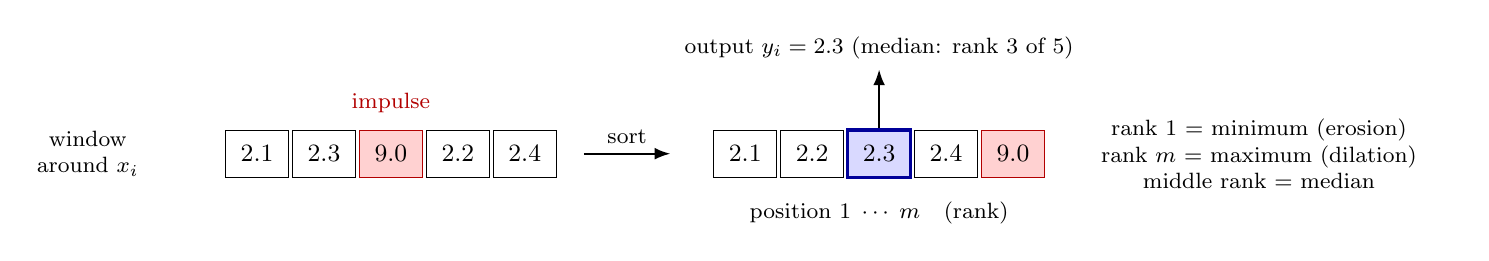
\begin{tikzpicture}[
  cell/.style={draw, minimum width=8mm, minimum height=6mm, font=\small},
  bad/.style={cell, fill=red!18, draw=red!70!black},
  pick/.style={cell, fill=blue!15, draw=blue!60!black, very thick},
  lab/.style={font=\footnotesize, align=center},
  arr/.style={-{Latex[length=2mm]}, thick}]
  % input window
  \node[lab] at (-1.3,0) {window\\around $x_i$};
  \foreach \v [count=\k] in {2.1,2.3,9.0,2.2,2.4}{
    \ifnum\k=3 \node[bad] (a\k) at (\k*0.85,0) {\v};
    \else      \node[cell] (a\k) at (\k*0.85,0) {\v};\fi}
  \node[lab, red!70!black] at (2.55,0.65) {impulse};
  % sort
  \draw[arr] (5.0,0) -- node[above, lab]{sort} (6.1,0);
  \foreach \v [count=\k] in {2.1,2.2,2.3,2.4,9.0}{
    \ifnum\k=3 \node[pick] (s\k) at (6.2+\k*0.85,0) {\v};
    \else\ifnum\k=5 \node[bad] (s\k) at (6.2+\k*0.85,0) {\v};
    \else \node[cell] (s\k) at (6.2+\k*0.85,0) {\v};\fi\fi}
  \node[lab] at (8.75,-0.75) {position $1 \;\cdots\; m$\quad (rank)};
  % select
  \draw[arr] (s3.north) -- ++(0,0.75) node[above, lab]{output $y_i = 2.3$ (median: rank 3 of 5)};
  \node[lab, text width=4.9cm, anchor=west] at (11.0,0) {rank 1 = minimum (erosion)\\rank $m$ = maximum (dilation)\\middle rank = median};
\end{tikzpicture}
}
\caption{A rank filter. The window is sorted and one rank is selected. The impulse (9.0) is ignored.}\label{fig:median}
\end{figure}

Three properties make these filters attractive in practice:
\begin{itemize}\itemsep0pt
\item \textbf{No multiplications}: only comparisons, which are cheap in hardware.
\item \textbf{Robustness}: if any 2 of the 5 samples of a median filter are corrupted, however wildly, the output still
  stays within the range of the clean samples. This tolerance (the \emph{breakdown point}) is known in advance.
\item \textbf{Stability}: if the input changes by at most $\varepsilon$ everywhere, the output changes by at most
  $\varepsilon$ (the filter is \emph{1-Lipschitz}). This holds for any chain of rank filters, however long.
\end{itemize}
Their weakness is design. The output jumps from one sample to another when a parameter crosses a threshold, so the
derivative with respect to the parameters is zero almost everywhere and gradient descent cannot learn them.

%=====================================================================================================
\section{The 1993 structure: NEst}\label{sec:nest}
The thesis proposed a trainable stage, called NEst, that avoids the zero-gradient problem (Fig.~\ref{fig:nest}).
Each sample receives an offset $b_j$ before sorting, and the sorted values are combined with weights $h_k$:
\[
y_i=\sum_{k}|h_k|\,(z+b)_{(k)} ,
\]
where $(z+b)_{(k)}$ is the $k$-th smallest value of the window after adding the offsets. Because the offsets change the
\emph{values}, the output varies smoothly with them, and the thesis adapted cascades of two NEst stages with the
least-mean-squares (LMS) algorithm.

\begin{figure}[h]\centering
\resizebox{0.86\linewidth}{!}{% Fig. 2 -- the 1993 NEst stage: offsets on positions, weights on ranks
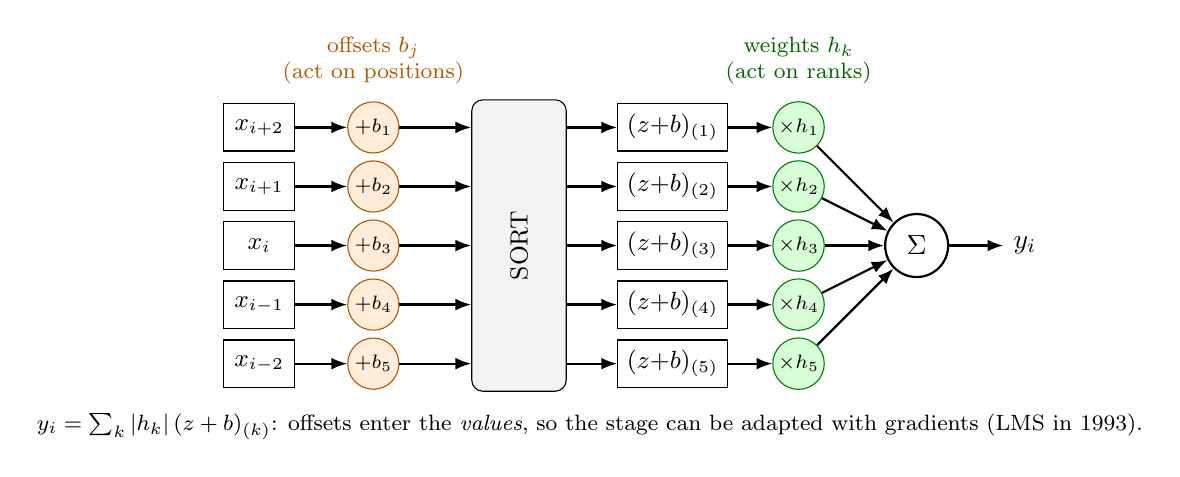
\begin{tikzpicture}[
  cell/.style={draw, minimum width=9mm, minimum height=6mm, font=\small},
  par/.style={draw, circle, inner sep=1pt, minimum size=6.5mm, font=\scriptsize, fill=orange!15, draw=orange!70!black},
  wpar/.style={draw, circle, inner sep=1pt, minimum size=6.5mm, font=\scriptsize, fill=green!15, draw=green!50!black},
  box/.style={draw, rounded corners, minimum height=37mm, minimum width=12mm, font=\small, fill=gray!10},
  lab/.style={font=\footnotesize, align=center},
  arr/.style={-{Latex[length=2mm]}, thick}]
  \foreach \t [count=\k] in {x_{i+2},x_{i+1},x_{i},x_{i-1},x_{i-2}}{
    \node[cell] (x\k) at (0,-\k*0.75) {$\t$};
    \node[par] (b\k) at (1.45,-\k*0.75) {$+b_{\k}$};
    \draw[arr] (x\k) -- (b\k);}
  \node[box] (S) at (3.3,-2.25) {\rotatebox{90}{SORT}};
  \foreach \k in {1,...,5}{\draw[arr] (b\k) -- (S.west |- b\k);}
  \foreach \k in {1,...,5}{
    \node[cell, minimum width=13mm] (z\k) at (5.25,-\k*0.75) {$(z{+}b)_{(\k)}$};
    \draw[arr] (S.east |- z\k) -- (z\k);
    \node[wpar] (h\k) at (6.85,-\k*0.75) {$\times h_{\k}$};
    \draw[arr] (z\k) -- (h\k);}
  \node[draw, circle, thick, minimum size=8mm] (sum) at (8.35,-2.25) {$\Sigma$};
  \foreach \k in {1,...,5}{\draw[arr] (h\k) -- (sum);}
  \draw[arr] (sum) -- ++(1.1,0) node[right]{$y_i$};
  \node[lab, orange!70!black] at (1.45,0.1) {offsets $b_j$\\(act on positions)};
  \node[lab, green!40!black] at (6.85,0.1) {weights $h_k$\\(act on ranks)};
  \node[lab] at (4.2,-4.55) {$y_i=\sum_k |h_k|\,(z+b)_{(k)}$: offsets enter the \emph{values}, so the stage can be adapted with gradients (LMS in 1993).};
\end{tikzpicture}
}
\caption{NEst stage (1993). Orange: offsets applied to window positions before sorting. Green: weights applied to the
sorted values. With one weight equal to 1 and zero offsets it is a plain rank filter; with several weights it averages
neighbouring ranks.}\label{fig:nest}
\end{figure}

Re-implemented today with exact gradients and the Adam optimiser, a NEst cascade reaches the noise floor on the thesis'
own example in 7\,s instead of 20\,s. However, when asked to recover 16 randomly chosen two-stage rank cascades, it
succeeds in only 2--3 of them: its parameters can imitate a rank filter only approximately.

%=====================================================================================================
\section{The proposal: WOS-R}\label{sec:wosr}
\subsection{Repetitions instead of masks}
We use the \emph{weighted order statistic} (WOS) filter \cite{brownrigg1984,yin1996}: each sample of the window is
copied $w_j$ times before sorting, and the output is the sample found at a fraction $r$ of the sorted list
(Fig.~\ref{fig:wosr}a,b). A large $w_j$ makes a position more influential; $w_j=0$ removes it; equal weights and
$r=\tfrac12$ give the median; $r$ near 0 or 1 gives erosion or dilation. The weights may be real numbers: any real
weights define the same filter as some set of integers. One stage with a 7-sample window has only 8 parameters.

\begin{figure}[h]\centering
\resizebox{\linewidth}{!}{% Fig. 3 -- one WOS-R stage: repetitions, exact selection at deployment, ramp during training
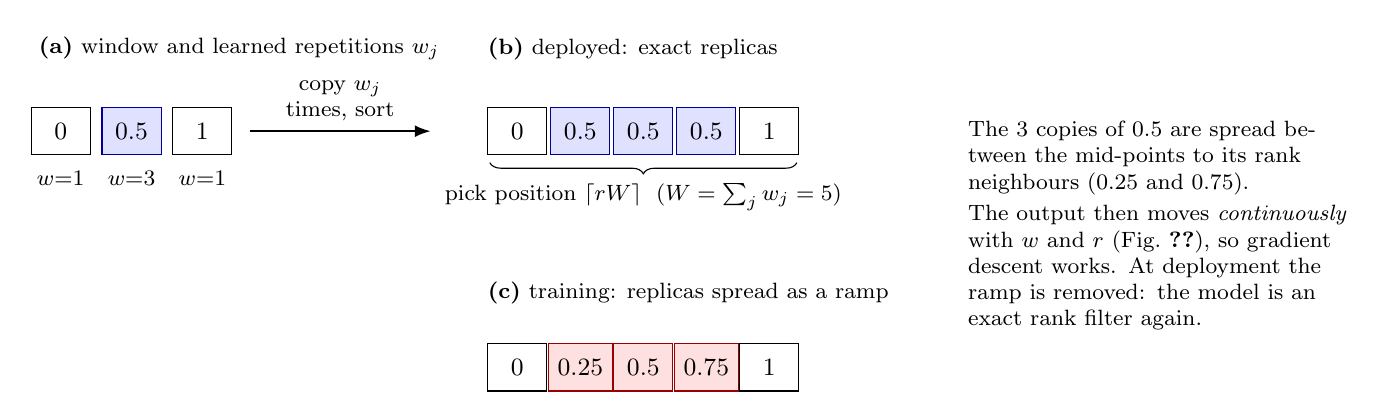
\begin{tikzpicture}[
  cell/.style={draw, minimum width=7.5mm, minimum height=6mm, font=\small},
  rep/.style={cell, fill=blue!12, draw=blue!60!black},
  ramp/.style={cell, fill=red!12, draw=red!60!black},
  pick/.style={very thick, draw=black},
  lab/.style={font=\footnotesize, align=center},
  arr/.style={-{Latex[length=2mm]}, thick}]
  % (a) input with repetition weights
  \node[lab, anchor=west] at (-0.4,1.05) {\textbf{(a)} window and learned repetitions $w_j$};
  \node[cell] (p1) at (0,0) {0};   \node[lab] at (0,-0.6) {$w{=}1$};
  \node[rep]  (p2) at (0.9,0) {0.5}; \node[lab] at (0.9,-0.6) {$w{=}3$};
  \node[cell] (p3) at (1.8,0) {1};   \node[lab] at (1.8,-0.6) {$w{=}1$};
  \draw[arr] (2.4,0) -- node[above, lab]{copy $w_j$\\times, sort} (4.7,0);
  % (b) deployed list
  \node[lab, anchor=west] at (5.3,1.05) {\textbf{(b)} deployed: exact replicas};
  \foreach \v/\s [count=\k] in {0/cell,0.5/rep,0.5/rep,0.5/rep,1/cell}{\node[\s] (d\k) at (5.0+\k*0.8,0) {\v};}
  \draw[decorate, decoration={brace, amplitude=4pt, mirror}] (5.45,-0.4) -- (9.35,-0.4)
     node[midway, below=4pt, lab]{pick position $\lceil rW\rceil$ \;($W=\sum_j w_j=5$)};
  % (c) training list
  \node[lab, anchor=west] at (5.3,-2.05) {\textbf{(c)} training: replicas spread as a ramp};
  \foreach \v/\s [count=\k] in {0/cell,0.25/ramp,0.5/ramp,0.75/ramp,1/cell}{\node[\s] (t\k) at (5.0+\k*0.8,-3.0) {\v};}
  \node[lab, text width=5.0cm, align=left, anchor=west] at (11.4,-1.2) {The 3 copies of 0.5 are spread between the mid-points to its rank neighbours (0.25 and 0.75).\\[2pt]
     The output then moves \emph{continuously} with $w$ and $r$ (Fig.~\ref{fig:rampcurve}), so gradient descent works.
     At deployment the ramp is removed: the model is an exact rank filter again.};
\end{tikzpicture}
}
\caption{One WOS-R stage. (a) Each sample carries a learned repetition weight. (b) At deployment the copies are exact
and one position of the sorted list is selected. (c) During training the copies are spread as a ramp between the
neighbouring sorted values.}\label{fig:wosr}
\end{figure}

\subsection{The ramp: smooth for training, exact for deployment}
With exact copies, the output jumps between sample values when $r$ or $w$ change (blue curve in
Fig.~\ref{fig:rampcurve}): zero gradient almost everywhere. During training we therefore replace the copies of each
sample by a ramp that spans half the distance to its sorted neighbours (Fig.~\ref{fig:wosr}c). The output becomes a
continuous, piecewise-linear function of the parameters (red curve), and ordinary gradient descent works. After
training the ramp is switched off. The deployed model is again an exact rank filter, so the three properties of
Section~2 hold for the model that is actually used.

\begin{figure}[h]\centering
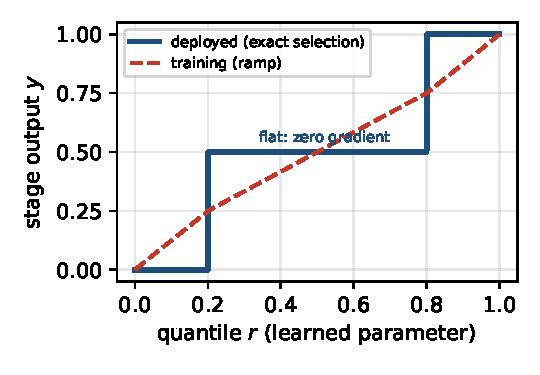
\includegraphics[width=0.52\linewidth]{figs/ramp_curve.pdf}
\caption{Output of the stage of Fig.~\ref{fig:wosr} as the quantile $r$ changes: staircase at deployment, continuous
ramp during training.}\label{fig:rampcurve}
\end{figure}

\subsection{Cascade or bank?}\label{sec:arch}
Stages can be combined in two ways (Fig.~\ref{fig:arch}, Table~\ref{tab:arch}).

\textbf{Cascade.} Stages are applied one after the other, as in the 1993 thesis. The output is always one of the input
samples; the model uses no multiplications and keeps every guarantee. It can express openings, closings, medians of
medians and any chain of weighted medians.

\textbf{Bank.} $C$ small cascades run in parallel on the same input, and their outputs are combined by a weighted sum
$y=\sum_c a_c\,y_c+b$. This costs $C$ multiplications per sample and buys expressiveness: the sum can subtract one
operator from another (for instance identity minus opening, the \emph{top-hat}) or average several rank filters.
Robustness is kept, but the stability bound becomes $\sum_c|a_c|$ instead of 1. One practical detail matters: a bank
must be trained with the ramp \emph{gradually} reduced to zero during training. Otherwise the weighted sum learns to
exploit the ramp itself, and the deployed bank can be very poor (20\,dB worse on a simple median).

\begin{figure}[h]\centering
\resizebox{0.95\linewidth}{!}{% Fig. 5 -- cascade (series) vs bank (parallel) of WOS-R stages
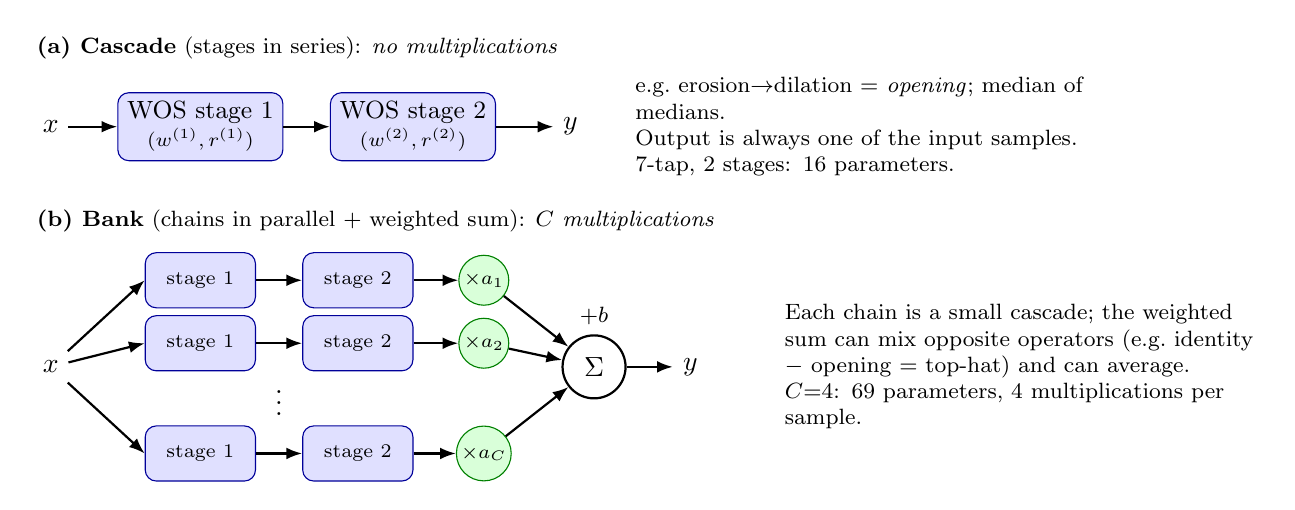
\begin{tikzpicture}[
  st/.style={draw, rounded corners, fill=blue!12, draw=blue!60!black, minimum width=17mm, minimum height=7mm, font=\small, align=center},
  lab/.style={font=\footnotesize, align=center},
  arr/.style={-{Latex[length=2mm]}, thick}]
  % ---------------- cascade
  \node[lab, anchor=west] at (-0.6,1.0) {\textbf{(a) Cascade} (stages in series): \emph{no multiplications}};
  \node (xin) at (-0.3,0) {$x$};
  \node[st] (c1) at (1.6,0) {WOS stage 1\\[-1pt]\scriptsize $(w^{(1)},r^{(1)})$};
  \node[st] (c2) at (4.3,0) {WOS stage 2\\[-1pt]\scriptsize $(w^{(2)},r^{(2)})$};
  \node (yout) at (6.3,0) {$y$};
  \draw[arr] (xin) -- (c1); \draw[arr] (c1) -- (c2); \draw[arr] (c2) -- (yout);
  \node[lab, text width=6.0cm, align=left, anchor=west] at (7.0,0) {e.g.\ erosion$\to$dilation = \emph{opening}; median of medians.\\
     Output is always one of the input samples. 7-tap, 2 stages: 16 parameters.};
  % ---------------- bank
  \node[lab, anchor=west] at (-0.6,-1.2) {\textbf{(b) Bank} (chains in parallel + weighted sum): \emph{$C$ multiplications}};
  \node (xb) at (-0.3,-3.05) {$x$};
  \foreach \c/\yy in {1/-1.95,2/-2.75,C/-4.15}{
    \node[st, minimum width=14mm] (b1\c) at (1.6,\yy) {\scriptsize stage 1};
    \node[st, minimum width=14mm] (b2\c) at (3.6,\yy) {\scriptsize stage 2};
    \draw[arr] (xb) -- (b1\c.west); \draw[arr] (b1\c) -- (b2\c);
    \node[draw, circle, inner sep=1pt, minimum size=6mm, font=\scriptsize, fill=green!15, draw=green!50!black] (a\c) at (5.2,\yy) {$\times a_{\c}$};
    \draw[arr] (b2\c) -- (a\c);}
  \node at (2.6,-3.4) {$\vdots$};
  \node[draw, circle, thick, minimum size=8mm] (S) at (6.6,-3.05) {$\Sigma$};
  \foreach \c in {1,2,C}{\draw[arr] (a\c) -- (S);}
  \draw[arr] (S) -- ++(1.0,0) node[right]{$y$};
  \node[lab] at (6.6,-2.4) {$+b$};
  \node[lab, text width=6.0cm, align=left, anchor=west] at (8.9,-3.05) {Each chain is a small cascade; the weighted sum can mix opposite operators
     (e.g.\ identity $-$ opening = top-hat) and can average.\\ $C{=}4$: 69 parameters, 4 multiplications per sample.};
\end{tikzpicture}
}
\caption{The two layouts used in this work.}\label{fig:arch}
\end{figure}

\begin{table}[h]\centering\small
\caption{Cascade versus bank (1D, 7-sample windows, two stages per chain).}\label{tab:arch}
\begin{tabularx}{\linewidth}{@{}l>{\raggedright\arraybackslash}X>{\raggedright\arraybackslash}X@{}}\toprule
 & \textbf{Cascade} & \textbf{Bank of $C$ chains} \\\midrule
Structure & stages in series & $C$ cascades in parallel + weighted sum \\
Parameters & 16 & 69 ($C{=}4$), 137 ($C{=}8$) \\
Multiplications per sample & 0 & $C$ \\
Output & always one input sample & weighted combination of $C$ selected samples \\
Guarantees & robustness, stability bound 1, no multiplications & robustness; stability bound $\sum_c|a_c|$ \\
Can represent & medians, erosion/dilation, openings, weighted medians & the same, plus signed combinations (top-hat) and coarse averaging \\
Training & ramp on, then switched off & ramp reduced gradually to zero \\
Error on 1D impulses & $-18.7\pm1.3$\,dB over 20 trainings (best $-20.7$) & $-21.1\pm0.5$\,dB over 6 trainings ($C{=}8$)\\
Sensitivity to initialisation & high: use a few restarts & low \\
\bottomrule\end{tabularx}
\end{table}

%=====================================================================================================
\section{How does it compare with neural networks?}\label{sec:results}
We ran five tests on a 2-core CPU, comparing WOS-R with residual CNNs (small, medium and large), MLPs and small
Transformers trained on the same data with the same loss. Table~\ref{tab:summary} gives the headline numbers; full
tables are in the Appendix.

\begin{itemize}\itemsep1pt
\item \textbf{B1 -- 1D signals with impulses.} Error in dB (lower is better; $-20$\,dB means the remaining error has 1\,\%
  of the signal energy). The best bank ($-21.1$\,dB, 137 parameters) is 1.2\,dB behind the best CNN (22\,081
  parameters). A single 16-parameter cascade is less reliable: $-18.7\pm1.3$\,dB over 20 independent trainings; keeping
  the best of 4 short restarts (chosen on validation data) gives $-19.6$\,dB, on a par with a 3\,857-parameter CNN
  ($-19.4$\,dB). When the impulses become twice
  as large as in training, the rank models degrade least and the Transformer breaks down.
\item \textbf{B2 -- What can each model represent?} We asked every model to imitate eleven known operators. When WOS-R
  finds a rank-type target it reproduces it \emph{exactly}, which no network does; it cannot represent operators that need
  subtraction or squaring, which networks learn easily (Fig.~\ref{fig:b2}).
\item \textbf{B3 -- Images with salt-and-pepper noise.} Quality in PSNR (peak signal-to-noise ratio, dB, higher is
  better) on 68 standard test photographs. A \emph{switching} WOS-R, applied only to pixels that look like impulses, uses
  52 parameters and is 0.5\,dB behind a 74\,593-parameter DnCNN at 50\,\% corrupted pixels. With a different kind of
  impulse never seen in training, the plain WOS-R is 5.6--6.7\,dB \emph{better} than the DnCNN (Fig.~\ref{fig:qual}).
\item \textbf{B4 -- Radar detection.} A constant-false-alarm-rate (CFAR) detector decides whether a target is present
  from the surrounding range cells. A 34-parameter WOS-R is the best detector whenever other targets contaminate those
  cells; an MLP loses up to 4.3\,dB and a Transformer stops detecting. Without interferers, the MLP is 0.3\,dB better.
\item \textbf{B5 -- Federated learning with faulty nodes.} Twenty devices train a shared model and four send corrupted
  updates. A cascade of rank operations over time and over nodes keeps 75\,\% accuracy in the worst case (54\,\% when the
  devices hold very different data); a learned
  aggregator alone collapses to chance (10\,\%), but works well \emph{after} the rank cascade.
\end{itemize}

\begin{table}[t]\centering\small
\caption{Headline results: best WOS-R against the best network in each test (from the Appendix tables).}\label{tab:summary}
\setlength{\tabcolsep}{4pt}
\begin{tabularx}{\linewidth}{@{}>{\raggedright\arraybackslash}p{3.1cm}lrlr>{\raggedright\arraybackslash}X@{}}\toprule
Test & WOS-R (params) & score & Network (params) & score & Verdict\\\midrule
B1 impulses, 1D (dB, $\downarrow$) & bank (137) & $-21.1$ & CNN (22\,081) & $-22.3$ & 161$\times$ smaller, 1.2\,dB worse\\
B1 impulses $\times2$ (OOD) & bank (137) & $-17.8$ & CNN (22\,081) & $-17.4$ & WOS-R better; Transformer fails ($+0.3$)\\
B1 Gaussian noise & bank (137) & $-18.2$ & CNN (22\,081) & $-20.4$ & network better\\
B3 salt \& pepper 50\,\% (PSNR, $\uparrow$) & switching (52) & 26.22 & DnCNN (74\,593) & 26.74 & 1\,434$\times$ smaller, 0.5\,dB worse\\
B3 random impulses (OOD) & cascade (52) & 24.46 & DnCNN (74\,593) & 17.74 & WOS-R +6.7\,dB\\
B4 radar, 8 interferers (SNR needed, $\downarrow$) & WOS-R (34) & 17.09 & MLP (6\,337) & 20.35 & WOS-R +3.3\,dB\\
B5 federated, worst case (accuracy) & rank cascade (0) & 0.753 & learned (5\,569) & 0.100 & learned only works after a rank cascade\\
\bottomrule\end{tabularx}
\end{table}

\paragraph{Benchmark dashboards.} Figures~\ref{fig:bench1d}--\ref{fig:benchacc} show, for every model, the residual
error in the training conditions and in unseen conditions, the number of parameters, the multiplications per output, the
CPU latency, the training curves and the time needed to converge. Colour marks the family: blue for rank-based models,
orange for neural networks, green for classical filters. Three observations stand out. First, the rank models sit at
the left of every cost axis (16--213 parameters, 0--8 multiplications) while staying within about 1\,dB of the best
network in the training conditions. Second, their error moves least when the conditions change (short segments in
Figs.~\ref{fig:bench1d}a and \ref{fig:benchimg}a). Third, they converge in 15--90\,s: WOS-R starts as a median
filter, which is already a reasonable denoiser, so its training curve starts low (Fig.~\ref{fig:bench1d}e). Their
latency in PyTorch is not lower than that of small CNNs, because sorting is not what CPUs and deep-learning libraries
are optimised for.

\begin{figure}[p]\centering
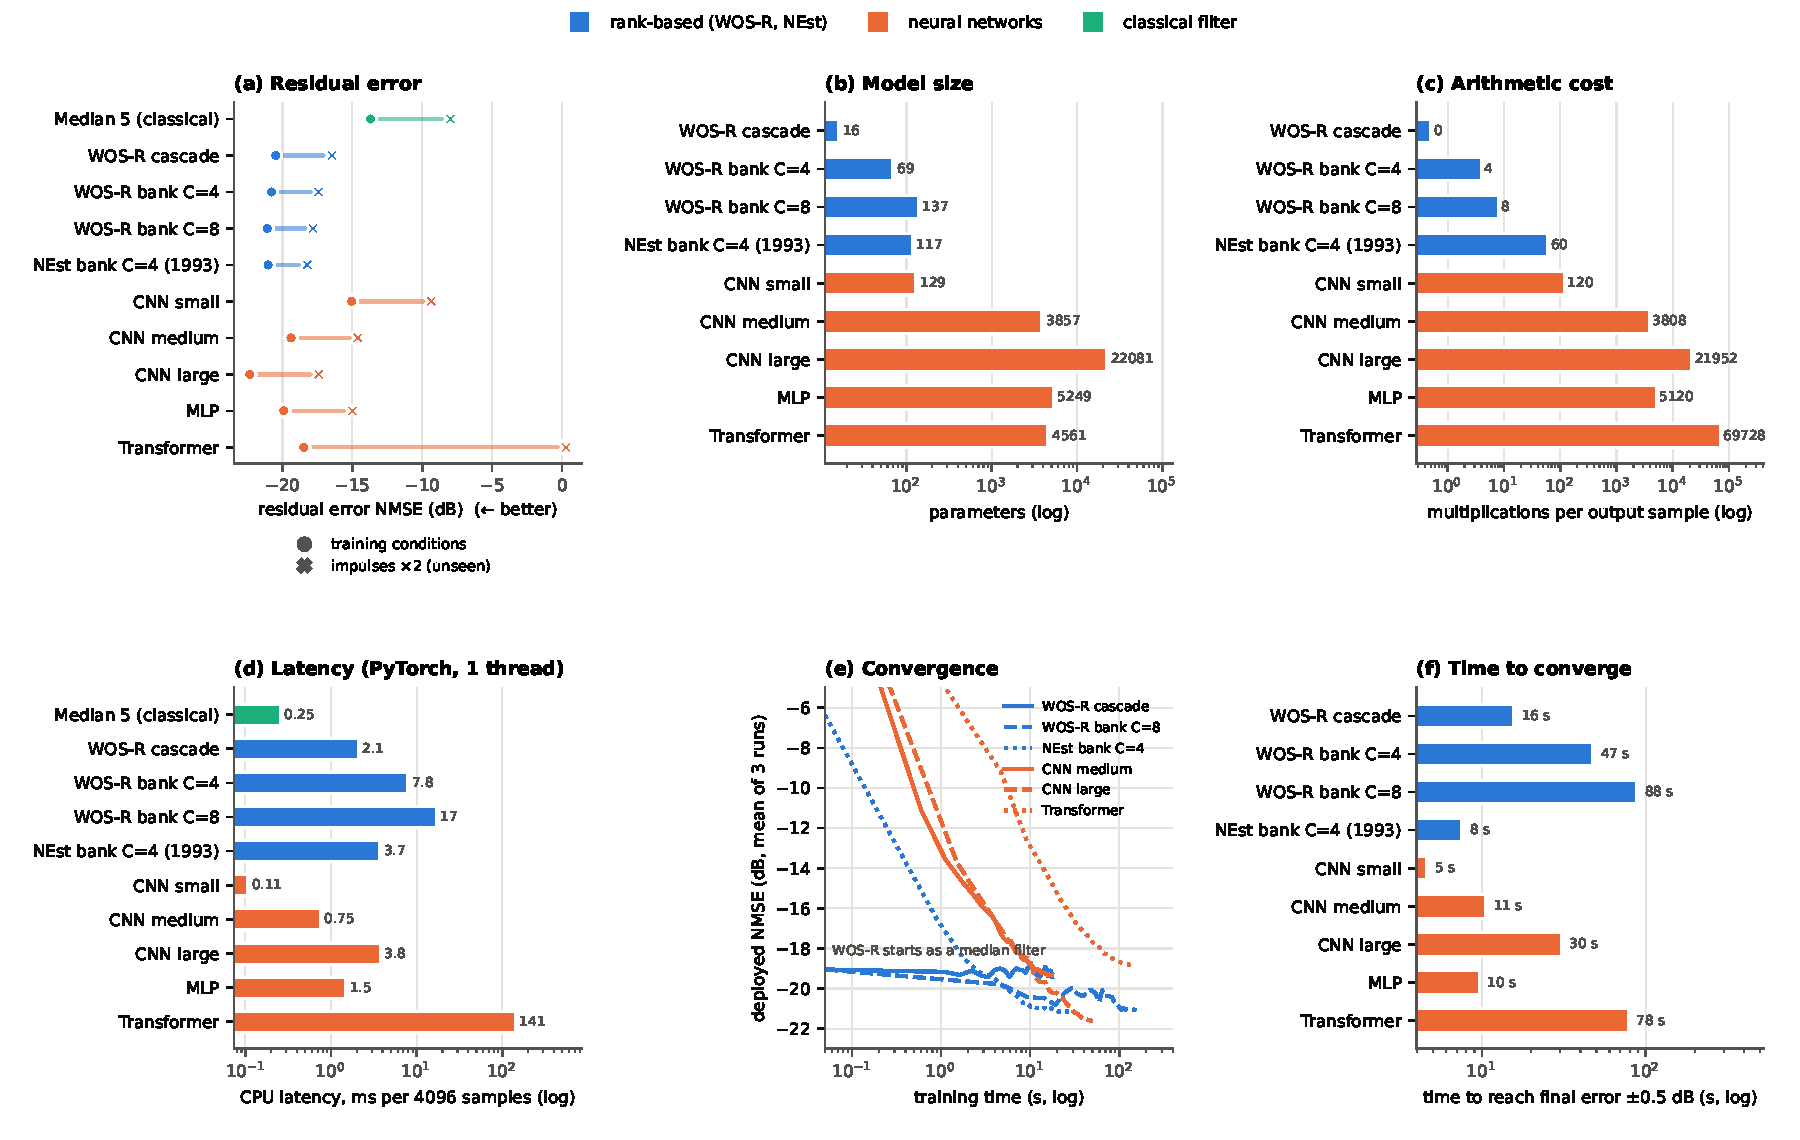
\includegraphics[width=\linewidth]{figs/bench_1d.pdf}
\caption{1D impulsive denoising (B1). (a) Residual error (normalised mean squared error, NMSE; lower is better) in
training conditions (o) and with impulses twice as large (x). (b) Parameters. (c) Multiplications per output sample.
(d) CPU latency. (e) Error of the deployed model during training against training time (3 runs). (f) Time until the
error stays within 0.5\,dB of its final value.}\label{fig:bench1d}
\end{figure}

\begin{figure}[t]\centering
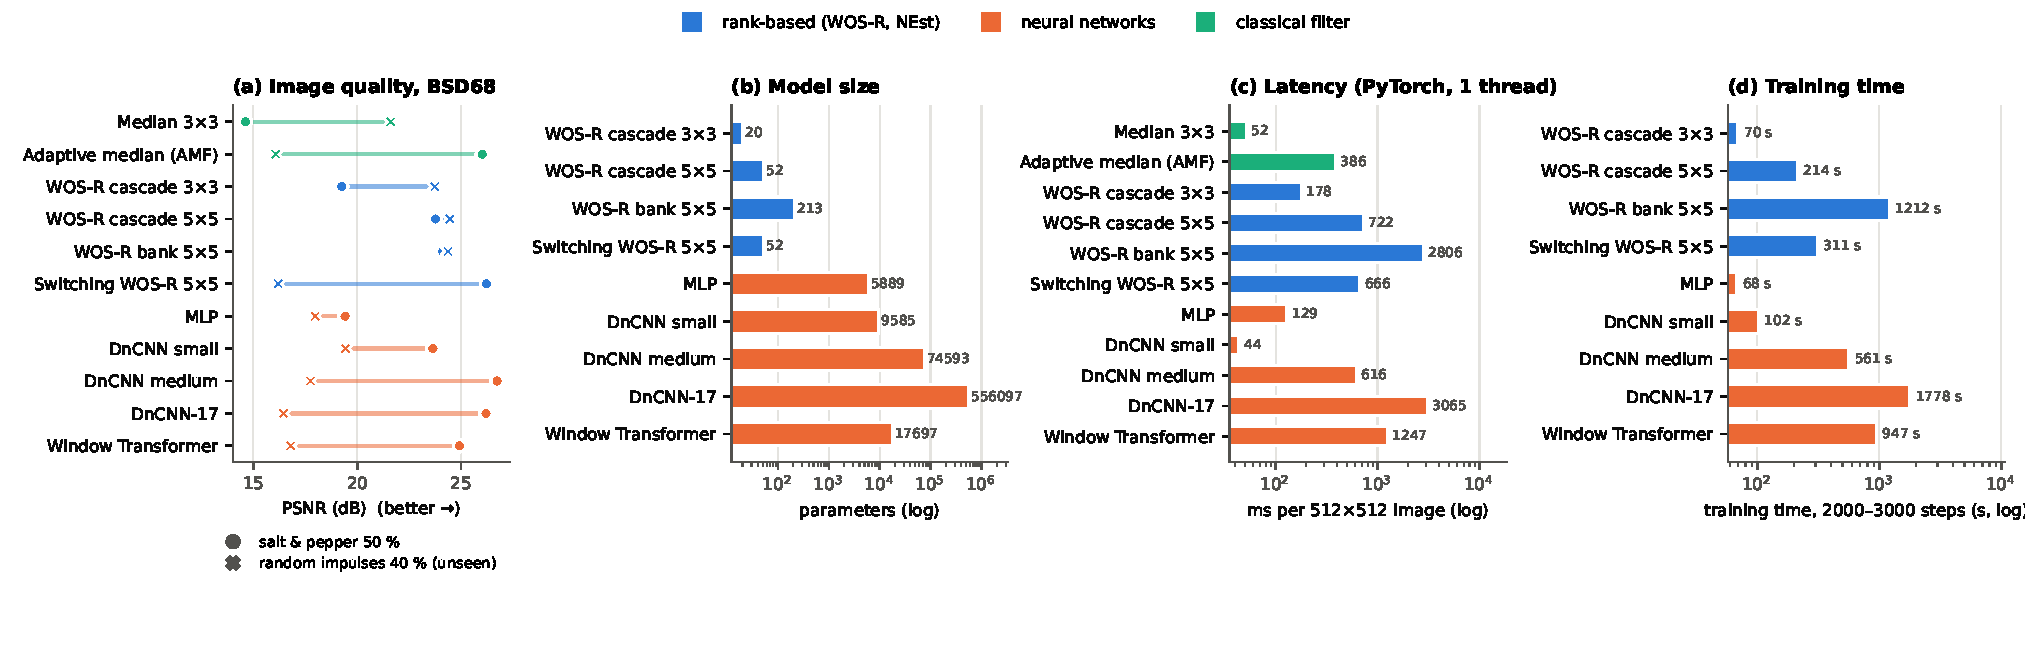
\includegraphics[width=\linewidth]{figs/bench_img.pdf}
\caption{Image impulse denoising on 68 test photographs (B3). (a) Image quality (PSNR, higher is better) with 50\,\%
salt-and-pepper pixels (o, seen in training) and 40\,\% random-valued impulses (x, never seen). (b) Parameters. (c) CPU
latency per $512{\times}512$ image. (d) Training time.}\label{fig:benchimg}
\end{figure}

\begin{figure}[t]\centering
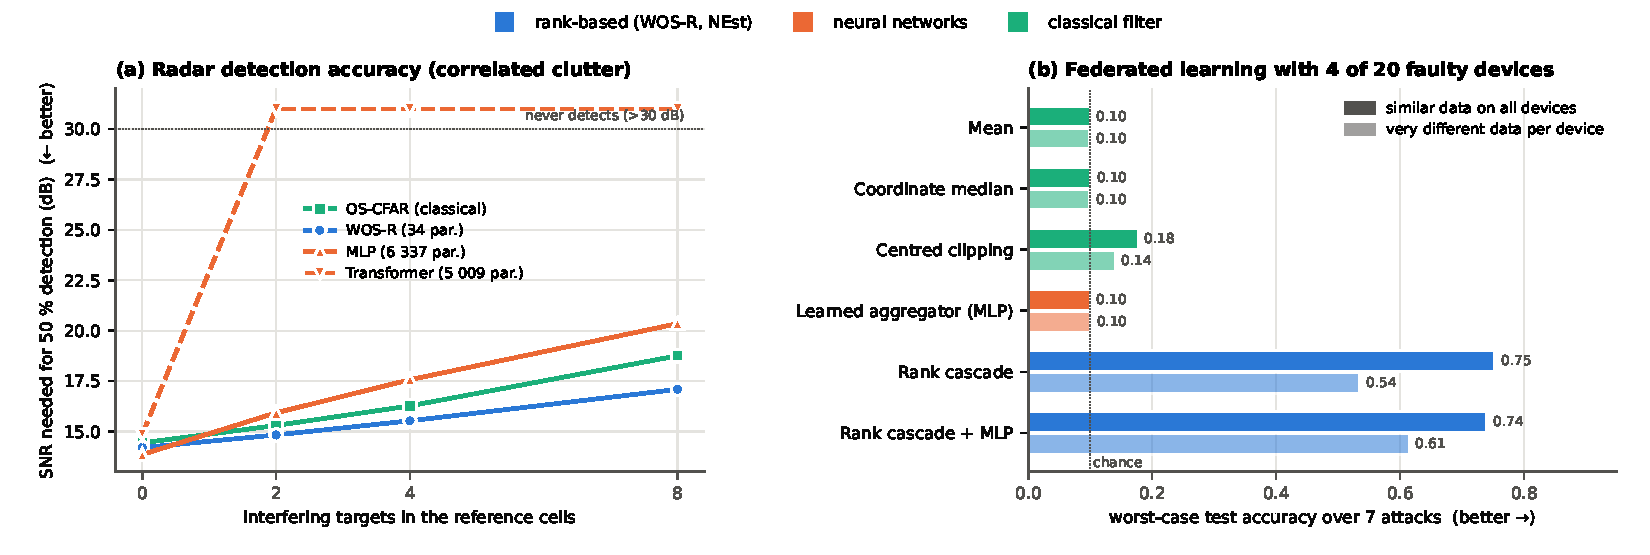
\includegraphics[width=\linewidth]{figs/bench_acc.pdf}
\caption{Accuracy in the two decision tasks. (a) Radar detection (B4): signal-to-noise ratio needed to detect half of
the targets as interfering targets are added (lower is better; the Transformer never reaches 50\,\% with interferers).
(b) Federated learning (B5): worst test accuracy over seven types of faulty devices.}\label{fig:benchacc}
\end{figure}

\begin{figure}[t]\centering
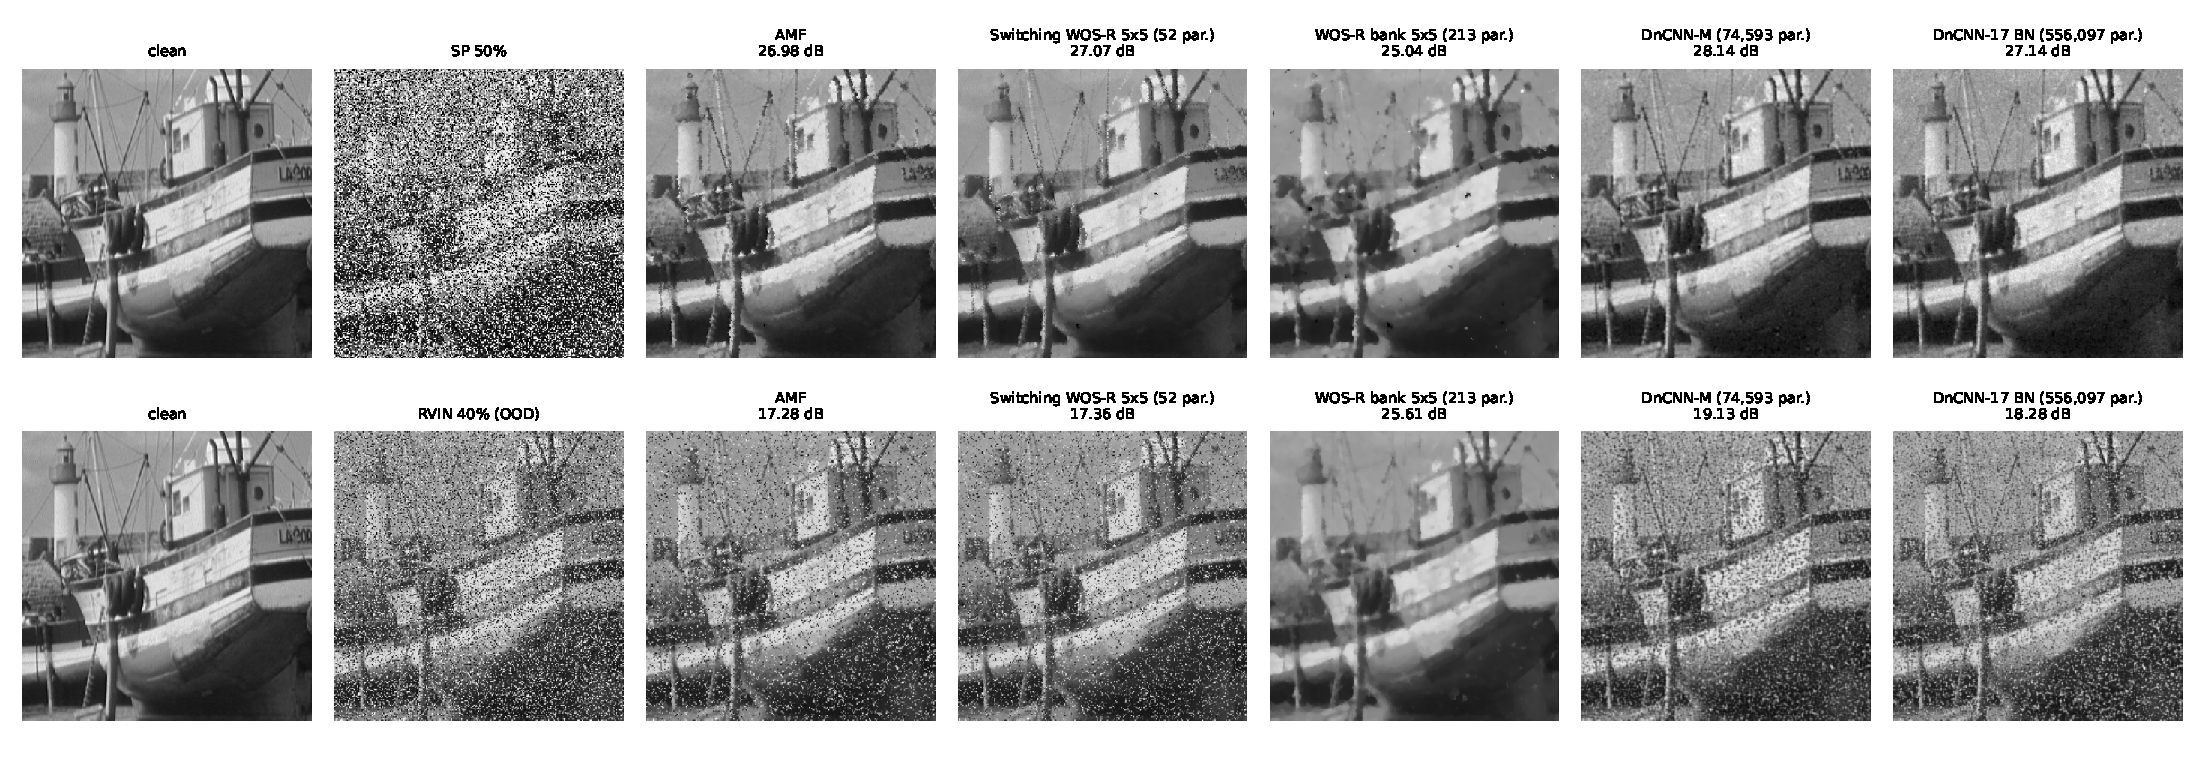
\includegraphics[width=\linewidth]{figs/qual.pdf}
\caption{Image test (``boat'', crop). Top: 50\,\% salt-and-pepper pixels (seen in training). Bottom: 40\,\% random-valued
impulses (never seen). AMF is the classical adaptive median filter. Numbers are PSNR of the full image.}\label{fig:qual}
\end{figure}

\paragraph{Cost.} The savings are in operations: 0 to 8 multiplications per sample instead of 6\,000--74\,000, replaced
by a few hundred comparisons. With standard PyTorch code, which is optimised for convolutions, WOS-R is not faster on a
CPU (1.1--4.5 times slower); the gain would come from comparator hardware such as FPGAs or low-power DSPs.

%=====================================================================================================
\section{Are stages and window size hyper-parameters?}\label{sec:struct}
In the experiments above they were fixed by hand (for instance 2 stages of 7 samples). They do not have to be: the
\emph{maximum} depth, window and bank size are hyper-parameters, but the structure actually used can be learned during
training without leaving the rank-filter family, because every unnecessary piece has a natural ``off'' state:
\begin{itemize}\itemsep0pt
\item a \textbf{stage} becomes the identity when the weight of its centre sample exceeds the larger of $r$ and $1-r$
  (the centre is then always selected), so it can simply be removed;
\item a \textbf{tap} disappears when its repetition weight goes to zero, which shortens the window;
\item a \textbf{chain} of a bank disappears when its mixing weight $a_c$ goes to zero.
\end{itemize}
We trained an over-sized cascade (4 stages of 9 samples, extra stages starting as the identity) with two small
penalties that push stages towards the identity and weights towards zero, then removed every stage and tap whose
removal did not change the error on separate validation data (Table~\ref{tab:struct}).

\begin{table}[h]\centering\small
\caption{Structure learned from an over-sized cascade (4 stages $\times$ 9 samples). Error above the best achievable,
in dB; 2 training runs per target (3 for B1).}\label{tab:struct}
\begin{tabularx}{\linewidth}{@{}l>{\raggedright\arraybackslash}X>{\raggedright\arraybackslash}X>{\raggedright\arraybackslash}X@{}}\toprule
Target & True structure & Learned structure & Result\\\midrule
Median of 7 & 1 stage, 7 samples & 1 stage, 7 samples (all runs) & exact (0.0\,dB)\\
Opening (erosion$\to$dilation) & 2 stages of 5 & 3--4 smaller stages, equivalent & exact in 3 of 4 runs; the fixed 2$\times$7 cascade never found it\\
Rank cascade \#1 & median of 5, then erosion of 3 & 2 stages, the second an erosion of 3 & exact in 2 of 4 runs\\
1D impulses (B1) & unknown & 1--2 stages, 10--16 parameters & $-19.1$\,dB (fixed 2$\times$7: $-18.7$)\\
Bank of 8 chains (B1) & unknown & 6--7 chains kept & no loss ($-20.8$\,dB)\\
\bottomrule\end{tabularx}
\end{table}

\begin{figure}[h]\centering
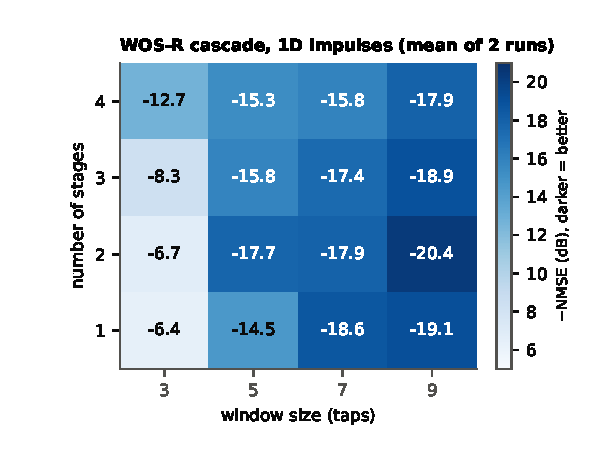
\includegraphics[width=0.48\linewidth]{figs/struct_grid.pdf}
\caption{Hand-tuning the same two hyper-parameters: error of a WOS-R cascade on 1D impulses for every combination of
depth and window (darker is better).}\label{fig:grid}
\end{figure}

Two lessons follow. The structure can be learned: the median and the second stage of cascade \#1 are recovered
exactly, and the B1 model shrinks to 1--2 stages without losing accuracy. More surprisingly, \emph{starting larger
helps the optimiser}: the opening, which the fixed 2-stage cascade never found, is found by the over-sized one as an
equivalent chain of smaller filters. For comparison, a plain grid search over depth and window
(Fig.~\ref{fig:grid}) costs 16 trainings (one per configuration) and still depends on luck: deeper cascades started at random get worse, and a
single 2$\times$7 cascade varies by up to 4\,dB between runs. Since one training takes about 20\,s, the practical recipe
is: start over-sized with extra stages at the identity, prune, and keep the best of a few restarts.

%=====================================================================================================
\section{When should you use it?}
\begin{table}[h]\centering\small
\begin{tabularx}{\linewidth}{@{}>{\raggedright\arraybackslash}X>{\raggedright\arraybackslash}X@{}}\toprule
\textbf{WOS-R is a good choice} & \textbf{A neural network is a better choice}\\\midrule
impulsive or heavy-tailed noise, especially of unknown size or type & Gaussian noise at the level seen in training\\
radar detection with interfering targets & more corrupted samples than the filter can tolerate\\
robust aggregation of data from unreliable sources (as a front-end) & operators that need subtraction or squaring\\
very small budgets: ${<}\,250$ parameters, almost no multiplications & highest possible accuracy with GPU training\\
\bottomrule\end{tabularx}
\end{table}

A practical recipe that emerges from the tests is \emph{rank first, learn second}: a WOS-R cascade bounds the influence
of corrupted inputs, and a small learned model placed after it adds accuracy.

\paragraph{Limitations.} All training ran on a CPU, images used a single training run per model, and the networks are
smaller and less trained than published GPU models, so their accuracy in the training conditions is underestimated.
The radar data are simulated. Training does not always find the best rank filter: a fixed two-stage cascade recovered
9 of 16 random cascades (against 2--3 for NEst), and a single cascade is sensitive to its random start
(Sec.~\ref{sec:struct}); banks and over-sized cascades are much more reliable.

\section{Conclusion}
A forty-year-old family of filters becomes trainable with a simple device: let each sample be a ramp while learning,
and a single sample when deployed. The resulting models are tiny, need almost no multiplications, keep provable
robustness, and hold their own against neural networks hundreds of times larger, above all when the data change. They
are not general approximators; combining them with small linear or learned stages is the natural next step.

\paragraph{Code and data.} All code, result files and a detailed technical version of this work are available with
this preprint.

\paragraph{Acknowledgement.} To Philippe Salembier, who supervised the 1993 thesis that started this work.

\bibliographystyle{unsrtnat}
\bibliography{refs}

%=====================================================================================================
\clearpage
\appendix
\section{Detailed results}
Abbreviations in the tables: SP salt-and-pepper; RVIN random-valued impulse noise; OOD out of distribution; NMSE
normalised mean squared error; PSNR peak signal-to-noise ratio; SSIM structural similarity (0--1, higher is better);
AMF adaptive median filter; CNN-S/M/L small/medium/large CNN; CFAR constant false-alarm rate; $P_d$, $P_{fa}$
probability of detection / false alarm; CW coordinate-wise; NNM nearest-neighbour mixing; AMO adaptive minimax ordered
weighted average; Med$_t$3 temporal median of the last 3 updates; ALIE ``a little is enough'' attack; IPM inner-product
manipulation attack; SDC silent data corruption. Mults and Comps: multiplications and comparisons per output sample.
``Ramp only'' rows are banks trained without the gradual reduction of the ramp (Sec.~\ref{sec:arch}).

\begin{table*}[t]\centering\small
\caption{B1: 1D restoration, normalised mean squared error (NMSE) in dB (mean $\pm$ std over 3 seeds; lower is better). Impulsive models are trained with 10\,\% impulses; OOD (out-of-distribution) columns change impulse rate or amplitude. NEst: 1993 thesis structure; CNN-S/M/L: small/medium/large residual CNN. Gaussian models are trained with $\sigma=0.2$. Params, multiply--accumulates and comparisons per output sample; ms: CPU latency for 4096 samples (1 thread). Best per column in bold.}\label{tab:b1}
\resizebox{\linewidth}{!}{\begin{tabular}{lrrrr|ccc|cc}\toprule
& & & & & \multicolumn{3}{c|}{Impulsive} & \multicolumn{2}{c}{Gaussian}\\
Model & Params & Mults & Comps & ms & in-dist & OOD $p{=}25\%$ & OOD $\times2$ & $\sigma{=}0.2$ & $\sigma{=}0.4$ (OOD)\\\midrule
Median 5 & 0 & 0 & 15 & 0.3 & $-13.7\pm1.2$ & $-3.6\pm0.3$ & $-8.0\pm1.3$ & $-14.9\pm0.3$ & $-8.9\pm0.4$\\
WOS-R chain $2{\times}7$ & 16 & 0 & 42 & 2.1 & $-20.5\pm0.1$ & $-11.3\pm0.3$ & $-16.5\pm1.7$ & $-16.4\pm0.3$ & $-11.1\pm0.4$\\
WOS-R bank $C{=}4$ & 69 & 4 & 168 & 7.8 & $-20.8\pm0.5$ & $-12.1\pm0.5$ & $-17.4\pm1.1$ & $-17.9\pm0.2$ & $-12.4\pm0.4$\\
WOS-R bank $C{=}8$ & 137 & 8 & 336 & 16.9 & $-21.1\pm0.6$ & $-12.4\pm0.6$ & $-17.8\pm0.9$ & $-18.2\pm0.4$ & $\mathbf{-12.7\pm0.4}$\\
\quad ablation: bank $C{=}4$, ramp only & 69 & 4 & 168 & 7.8 & $-19.9\pm0.9$ & $-11.1\pm1.6$ & $-16.1\pm1.4$ & -- & --\\
\quad ablation: bank $C{=}8$, ramp only & 137 & 8 & 336 & 16.9 & $-19.8\pm0.9$ & $-10.9\pm1.7$ & $-16.5\pm1.2$ & -- & --\\
NEst bank $C{=}4$ & 117 & 60 & 168 & 3.7 & $-21.0\pm0.4$ & $-12.3\pm0.3$ & $\mathbf{-18.2\pm0.9}$ & $-18.5\pm0.2$ & $-12.5\pm0.3$\\
CNN-S & 129 & 120 & 0 & 0.1 & $-15.0\pm0.7$ & $-8.3\pm0.2$ & $-9.4\pm0.9$ & $-19.1\pm0.3$ & $-11.3\pm0.3$\\
CNN-M & 3\,857 & 3\,808 & 0 & 0.7 & $-19.4\pm0.4$ & $-12.9\pm1.0$ & $-14.6\pm0.6$ & $-20.4\pm0.3$ & $-12.1\pm0.6$\\
CNN-L & 22\,081 & 21\,952 & 0 & 3.8 & $\mathbf{-22.3\pm0.6}$ & $\mathbf{-15.5\pm0.7}$ & $-17.4\pm0.0$ & $\mathbf{-20.4\pm0.2}$ & $-11.6\pm0.7$\\
MLP (window 15) & 5\,249 & 5\,120 & 0 & 1.5 & $-19.9\pm0.3$ & $-12.9\pm0.5$ & $-15.0\pm0.1$ & $-19.7\pm0.3$ & $-12.5\pm0.4$\\
Transformer & 4\,561 & 69\,728 & 0 & 141.0 & $-18.5\pm0.3$ & $-11.1\pm0.2$ & $0.3\pm0.3$ & $-16.5\pm0.3$ & $-9.6\pm0.4$\\
\bottomrule\end{tabular}}\end{table*}
\begin{table}[t]\centering\small
\caption{B2 coverage: excess normalised mean squared error (NMSE, dB) above the noise floor of the true operator (input $U[-5,5]$, SNR 35\,dB, mean of 2 seeds). Bold: $\le1$\,dB (operator represented); red: $>6$\,dB (not represented). Parameters in the last row.}\label{tab:b2}
\setlength{\tabcolsep}{4pt}\resizebox{\linewidth}{!}{\begin{tabular}{llrrrrrrr}\toprule
Target & Class & WOS-R chain & WOS-R bank 4 & bank 4, ramp only & NEst bank 4 & MLP & CNN-M & Transformer\\\midrule
Median 7 & rank & \textbf{0.0} & \textbf{0.0} & \textcolor{red!70!black}{19.8} & \textbf{0.1} & \textcolor{red!70!black}{16.8} & \textcolor{red!70!black}{18.9} & \textcolor{red!70!black}{26.2}\\
Flat erosion 5 & morphological & \textbf{0.0} & \textbf{0.0} & \textcolor{red!70!black}{20.6} & 3.3 & \textcolor{red!70!black}{6.5} & \textcolor{red!70!black}{9.5} & 5.5\\
Opening 5 & morph., 2 stages & \textcolor{red!70!black}{19.7} & \textcolor{red!70!black}{14.5} & \textcolor{red!70!black}{23.6} & 1.2 & \textcolor{red!70!black}{13.0} & \textcolor{red!70!black}{12.6} & \textcolor{red!70!black}{24.6}\\
WOS $(1,3,0,2,4,1,2)$ & WOS & \textbf{0.0} & \textbf{0.0} & \textcolor{red!70!black}{20.2} & \textcolor{red!70!black}{22.4} & \textcolor{red!70!black}{10.3} & \textcolor{red!70!black}{16.7} & \textcolor{red!70!black}{25.5}\\
Rank cascade \#1 & rank cascade & \textbf{0.0} & \textbf{0.0} & -- & \textbf{0.5} & \textcolor{red!70!black}{18.1} & \textcolor{red!70!black}{19.9} & \textcolor{red!70!black}{26.8}\\
Rank cascade \#12 & rank cascade & \textcolor{red!70!black}{19.8} & \textcolor{red!70!black}{12.3} & -- & \textcolor{red!70!black}{11.3} & \textcolor{red!70!black}{16.0} & \textcolor{red!70!black}{16.2} & \textcolor{red!70!black}{24.6}\\
Rank cascade \#5 & rank cascade & \textcolor{red!70!black}{25.2} & \textcolor{red!70!black}{21.4} & -- & \textcolor{red!70!black}{20.4} & \textcolor{red!70!black}{17.7} & \textcolor{red!70!black}{19.7} & \textcolor{red!70!black}{26.1}\\
Moving average 5 & linear, $h\ge0$ & \textcolor{red!70!black}{32.6} & \textcolor{red!70!black}{22.8} & -- & \textbf{0.8} & \textbf{0.8} & 1.1 & 2.3\\
High-pass $[-1,2,-1]/2$ & linear, signed & \textcolor{red!70!black}{30.3} & \textcolor{red!70!black}{24.4} & -- & \textbf{0.8} & \textbf{0.1} & \textbf{0.2} & \textbf{0.2}\\
Top-hat $x-$opening & non-increasing & \textcolor{red!70!black}{31.2} & \textcolor{red!70!black}{20.1} & -- & 2.0 & \textcolor{red!70!black}{11.2} & \textcolor{red!70!black}{7.9} & \textcolor{red!70!black}{23.4}\\
Point-wise $x^2/5$ & not translation-inv. & \textcolor{red!70!black}{29.6} & \textcolor{red!70!black}{26.2} & -- & \textcolor{red!70!black}{20.6} & 1.5 & 4.0 & \textbf{0.7}\\
\midrule Params & & 16 & 69 & 69 & 117 & 5\,249 & 3\,857 & 4\,561\\
\bottomrule\end{tabular}}\end{table}
\begin{figure}[h]\centering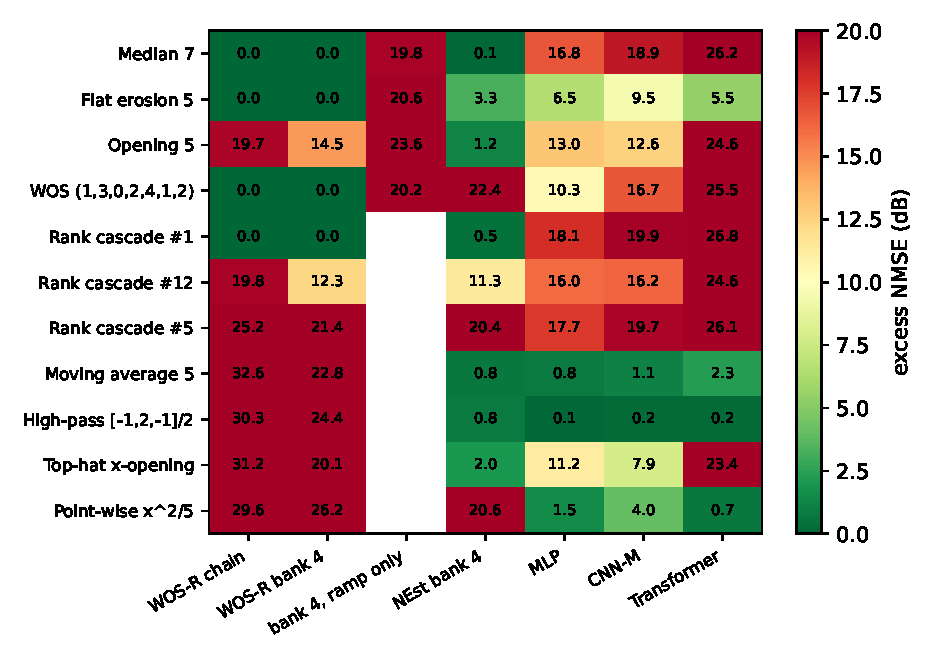
\includegraphics[width=0.62\linewidth]{figs/b2_coverage.pdf}
\caption{B2: how far each model stays from each target operator (dB above the best achievable; green represented,
red not represented).}\label{fig:b2}\end{figure}
\begin{table*}[t]\centering\small
\caption{B3: blind impulse denoising on BSD68, peak signal-to-noise ratio (PSNR, dB; higher is better) / structural similarity (SSIM). Training: salt-and-pepper (SP) with density $\sim U[0.1,0.6]$. Out of distribution (OOD): SP 70\,\%, random-valued impulse noise (RVIN). AMF: adaptive median filter; switching: WOS-R applied only to pixels that are an extreme of their $3{\times}3$ window. Mults and comparisons per pixel; latency in ms for a $512{\times}512$ image (1 CPU thread). Best per column in bold.}\label{tab:b3bsd68}
\resizebox{\textwidth}{!}{\begin{tabular}{lrrrr|cccc|cc}\toprule
Model & Params & Mults & Comps & ms & SP 10\% & SP 30\% & SP 50\% & SP 70\% & RVIN 20\% & RVIN 40\%\\\midrule
Median $3{\times}3$ & 0 & 0 & 36 & 52 & 28.26/0.851 & 21.94/0.682 & 14.62/0.268 & 9.58/0.069 & \textbf{26.70}/0.802 & 21.62/0.552\\
Median $5{\times}5$ & 0 & 0 & 125 & 149 & 25.79/0.731 & 24.90/0.711 & 21.49/0.617 & 13.48/0.226 & 25.36/0.718 & 23.59/0.637\\
Adaptive median (AMF, 7) & 0 & 0 & var. & 386 & 32.29/0.944 & 29.07/0.909 & 26.02/0.839 & 20.06/0.647 & 21.05/0.524 & 16.07/0.260\\
WOS-R $3{\times}3$, 2 stages & 20 & 0 & 72 & 178 & 27.37/0.812 & 25.50/0.774 & 19.25/0.562 & 11.90/0.154 & 26.63/0.793 & 23.73/0.668\\
WOS-R $5{\times}5$, 2 stages & 52 & 0 & 250 & 722 & 26.65/0.771 & 25.83/0.751 & 23.77/0.705 & 15.83/0.422 & 26.19/0.757 & \textbf{24.46}/0.696\\
WOS-R bank $C{=}4$ ($3{\times}3$) & 85 & 4 & 288 & 489 & 26.46/0.785 & 25.41/0.755 & 20.47/0.535 & 13.37/0.162 & 25.78/0.770 & 23.38/0.661\\
WOS-R bank $C{=}4$ ($5{\times}5$) & 213 & 4 & 1\,000 & 2806 & 26.60/0.770 & 25.89/0.752 & 24.11/0.699 & 16.85/0.372 & 26.07/0.756 & 24.37/0.696\\
\quad ablation: bank $C{=}4$ ($3{\times}3$), ramp only & 85 & 4 & 288 & 489 & 26.98/0.801 & 25.62/0.766 & 20.22/0.532 & 13.11/0.157 & 26.22/0.784 & 23.55/0.667\\
\quad ablation: bank $C{=}4$ ($5{\times}5$), ramp only & 213 & 4 & 1\,000 & 2806 & 26.74/0.776 & 25.98/0.757 & 24.08/0.704 & 16.55/0.369 & 26.20/0.762 & 24.43/0.700\\
Switching WOS-R $3{\times}3$ & 20 & 0 & 90 & 240 & 31.18/0.933 & 27.88/0.894 & 20.19/0.657 & 12.53/0.197 & 20.98/0.513 & 16.17/0.257\\
Switching WOS-R $5{\times}5$ & 52 & 0 & 268 & 666 & 30.52/0.923 & 28.88/0.902 & 26.22/0.840 & 18.48/0.604 & 20.89/0.505 & 16.19/0.253\\
Switching WOS-R bank $C{=}4$ ($3{\times}3$) & 85 & 4 & 306 & 726 & 29.78/0.885 & 27.76/0.843 & 21.87/0.602 & 14.82/0.218 & 20.82/0.501 & 16.11/0.253\\
MLP $5{\times}5$ & 5\,889 & 5\,760 & 0 & 129 & 30.09/0.892 & 24.37/0.642 & 19.42/0.384 & 15.44/0.200 & 21.87/0.513 & 17.98/0.317\\
DnCNN-S (6 layers, 16 ch) & 9\,585 & 9\,504 & 0 & 44 & 29.27/0.868 & 26.36/0.734 & 23.64/0.578 & 19.94/0.375 & 23.66/0.628 & 19.43/0.424\\
DnCNN-M (10 layers, 32 ch) & 74\,593 & 74\,304 & 0 & 616 & \textbf{33.65}/0.950 & \textbf{29.97}/0.881 & \textbf{26.74}/0.761 & \textbf{21.92}/0.521 & 22.08/0.530 & 17.74/0.336\\
DnCNN-17 (BN, 64 ch) & 556\,097 & 554\,112 & 0 & 3065 & 31.41/0.911 & 29.21/0.835 & 26.20/0.713 & 21.74/0.502 & 20.96/0.463 & 16.45/0.280\\
Window Transformer & 17\,697 & 25\,152 & 0 & 1247 & 30.37/0.915 & 28.01/0.834 & 24.92/0.681 & 20.17/0.437 & 20.28/0.447 & 16.80/0.291\\
\bottomrule\end{tabular}}\end{table*}
\begin{table}[t]\centering\small
\caption{B4: constant-false-alarm-rate (CFAR) detection in K-distributed clutter with range-correlated texture (AR(1) coefficient $\rho$), false-alarm probability $P_{fa}=10^{-4}$ calibrated per detector. Signal-to-noise ratio (SNR, dB) for detection probability $P_d=0.5$ with 0/2/4/8 interfering targets in the reference window (lower is better); learned detectors: mean of 2 seeds, trained with the same Neyman--Pearson objective.}\label{tab:b4}
\setlength{\tabcolsep}{4pt}\begin{tabular}{lr|cccc|cccc}\toprule
& & \multicolumn{4}{c|}{$\rho=0$} & \multicolumn{4}{c}{$\rho=0.9$}\\
Detector & Params & 0 & 2 & 4 & 8 & 0 & 2 & 4 & 8\\\midrule
OS-CFAR ($k{=}24$) & 0 & 15.46 & 16.41 & 17.33 & 19.91 & 14.43 & 15.30 & 16.27 & 18.75\\
GO-OS ($k{=}11$) & 0 & 15.76 & 16.63 & 17.50 & 20.09 & 14.91 & 15.72 & 16.50 & 18.85\\
WOS-R (32 repetitions) & 34 & 15.55 & \textbf{16.29} & \textbf{16.95} & \textbf{18.38} & 14.20 & \textbf{14.83} & \textbf{15.53} & \textbf{17.09}\\
MLP (log-equivariant) & 6\,337 & \textbf{15.22} & 17.64 & 19.37 & 22.69 & \textbf{13.86} & 15.92 & 17.57 & 20.35\\
Transformer (log-equivariant) & 5\,009 & 15.55 & $>30$ & $>30$ & $>30$ & 14.85 & $>30$ & $>30$ & $>30$\\
\bottomrule\end{tabular}\end{table}
\begin{table*}[t]\centering\small
\caption{B5: Byzantine/fault-robust aggregation (Fashion-MNIST, $n{=}20$ nodes, $f{=}4$ faulty, 300 steps, mean of 2 seeds). Test accuracy under each attack with heterogeneous data (Dirichlet $\alpha{=}0.1$), and worst case over attacks for $\alpha\in\{1,0.1\}$. CW: coordinate-wise; Med$_t$3: per-node temporal median of the last 3 submissions; NNM: nearest-neighbour mixing \cite{allouah2023}; AMO: adaptive minimax ordered weighted average (OWA). Attacks: ALIE (``a little is enough''), IPM (inner-product manipulation), burst-8 (faults persisting 8 steps), SDC (silent data corruption). $^\dagger$AMO uses a precomputed library of 5 OWA weight vectors (minimax second-order cone program), no training.}\label{tab:b5}
\resizebox{\linewidth}{!}{\begin{tabular}{lr|ccccccc|cc}\toprule
& & \multicolumn{7}{c|}{$\alpha=0.1$} & \multicolumn{2}{c}{worst case}\\
Aggregator & Params & none & sign-flip & ALIE & IPM & burst-8 & SDC & Gauss+burst & $\alpha{=}1$ & $\alpha{=}0.1$\\\midrule
Mean & 0 & 0.814 & 0.414 & 0.787 & 0.789 & 0.100 & 0.100 & 0.100 & 0.100 & 0.100\\
CW median & 0 & 0.603 & 0.599 & 0.565 & 0.465 & 0.244 & 0.683 & 0.100 & 0.100 & 0.100\\
CW trimmed mean & 0 & 0.728 & 0.642 & 0.728 & 0.372 & 0.100 & 0.707 & 0.100 & 0.100 & 0.100\\
NNM + CW trim & 0 & 0.793 & 0.727 & 0.714 & 0.695 & 0.100 & 0.803 & 0.100 & 0.100 & 0.100\\
Centred clipping & 0 & 0.806 & 0.681 & 0.771 & 0.693 & 0.707 & 0.803 & 0.141 & 0.177 & 0.141\\
AMO (minimax OWA) & 0$^\dagger$ & 0.591 & 0.551 & 0.610 & 0.410 & 0.247 & 0.602 & 0.100 & 0.100 & 0.100\\
Med$_t$3 $\to$ AMO & 0$^\dagger$ & 0.576 & 0.502 & 0.527 & 0.264 & 0.542 & 0.548 & 0.539 & 0.691 & 0.264\\
Med$_t$3 $\to$ NNM $\to$ CW trim & 0 & 0.779 & 0.672 & 0.772 & 0.535 & 0.782 & 0.773 & 0.762 & \textbf{0.753} & 0.535\\
Sorted-MLP aggregator & 5\,569 & 0.673 & 0.646 & 0.718 & 0.380 & 0.101 & 0.113 & 0.100 & 0.100 & 0.100\\
Med$_t$3 $\to$ NNM $\to$ sorted-MLP & 5\,569 & 0.777 & 0.703 & 0.767 & 0.615 & 0.780 & 0.775 & 0.773 & 0.740 & \textbf{0.615}\\
\bottomrule\end{tabular}}\end{table*}

\end{document}
